\documentclass[conference]{IEEEtran}
\IEEEoverridecommandlockouts

% Text, Language, and URLs
\usepackage[utf8]{inputenc}
\usepackage[english]{babel}
\usepackage[hyphens]{url}
\usepackage{cite}

% Math and Symbols
\usepackage{amsmath,amssymb,amsfonts}
\usepackage{textcomp}

% Figures, Subfigures, and Colors
\usepackage{float}
\usepackage{graphicx}
\usepackage{subcaption}
\usepackage[table]{xcolor}

% Tables and Formatting
\usepackage{multirow}
\usepackage{tabularx}
\usepackage{booktabs}
\usepackage{makecell}
\usepackage{diagbox}
\usepackage{multicol}
\usepackage{fancyhdr}
\usepackage{colortbl}
\usepackage{array}

% Custom Table Columns
\newcolumntype{L}{>{\raggedright\arraybackslash}X}
\newcolumntype{P}[1]{>{\centering\arraybackslash}m{#1}}

% Algorithms
\usepackage{algorithm}
\usepackage{algpseudocode}

% TikZ and PGFPlots
\usepackage{tikz}
\usetikzlibrary{positioning, arrows.meta}
\usepackage{pgfplots}
\pgfplotsset{compat=1.18}

\pagestyle{plain}

\makeatletter
\newcommand{\linebreakand}{%
  \end{@IEEEauthorhalign}
  \hfill\mbox{}\par
  \mbox{}\hfill\begin{@IEEEauthorhalign}
}
\makeatother

% ------------------------------------------------------------------
% Comparison-table cell markers (same convention as HERMES paper)
% ------------------------------------------------------------------
\definecolor{goodgreen}{RGB}{178,210,150}
\definecolor{atlasgreen}{RGB}{105,160,90}
\definecolor{badred}{RGB}{230,170,160}
\definecolor{nayellow}{RGB}{240,210,120}

\newcommand{\cmarkc}{\cellcolor{goodgreen}\textcolor{black!55}{\scriptsize$\checkmark$}}
\newcommand{\xmarkc}{\cellcolor{badred}\textcolor{black!40}{\scriptsize$\times$}}
\newcommand{\tmarkc}{\cellcolor{nayellow}\textcolor{black!65}{\scriptsize$\triangle$}}
\newcommand{\cmarkA}{\cellcolor{atlasgreen}\textcolor{white}{\textbf{\scriptsize$\checkmark$}}}

% ==================================================================
\begin{document}
\title{ATLAS: A Federated Multi-Task Framework for Privacy-Preserving Threat-Intelligence Estimation Across Regional Fusion Centers}

% \author{
% \IEEEauthorblockN{Kevin Kostage\IEEEauthorrefmark{1}, Chenqi Qu\IEEEauthorrefmark{2}, Alicia Morel\IEEEauthorrefmark{2}, Prasad Calyam\IEEEauthorrefmark{1}}
% \IEEEauthorblockA{\IEEEauthorrefmark{1}Department of Electrical Engineering and Computer Science, University of Missouri --- Columbia, USA. \\
% \IEEEauthorrefmark{2}Department of Computing and Software Engineering, Florida Gulf Coast University, USA. \\
% Email: \IEEEauthorrefmark{1}\{kskykn\}@umsystem.edu, \IEEEauthorrefmark{2}\{cqu,amorel\}@fgcu.edu, \IEEEauthorrefmark{1}{calyamp@missouri.edu}}
% }

\maketitle

% IEEE two-column layout has narrow columns; \sloppy lets LaTeX stretch
% inter-word spaces rather than overflowing the margin when a long
% \texttt{...} identifier (e.g. fairness_macro_f1_variance) lands at a
% line break. Slightly wider gaps in some lines, but no margin overruns.
\sloppy

\begin{abstract}
Regional fusion centers and similar inter-jurisdictional analytic units are responsible for fusing crime, infrastructure, and threat data from agencies that cannot share raw records due to statutory privacy constraints, agency policy, and population-level fairness obligations. Centralized analytics violate these constraints; isolated per-jurisdiction models lose the cross-regional signal that motivates the fusion-center mission in the first place. To address this tension, we present \textbf{ATLAS} (\textit{Adaptive Threat-intelligence Learning Across Sovereign jurisdictions}), a layered federated-learning framework that performs multi-task threat-class and escalation prediction across geographically partitioned fusion centers without raw-data sharing. ATLAS integrates three coordinated layers: (i) a privacy-preserving data-partitioning layer that enforces geographic non-IID splits and selectively removes statutorily sensitive features before any training begins; (ii) a multi-task FUSION-MLP layer with a shared trunk and two task heads (threat-class classification and escalation-score regression) optimized under a weighted joint loss; and (iii) a federated coordination layer supporting both single-process simulation (Ray-actor clients in one process) and real multi-node distributed gRPC operation, with FedAvg and FedProx aggregation strategies. We evaluate ATLAS through two complementary experiment groups: a learning-architecture group comparing centralized, local-only, and federated learning on the UCI Communities and Crime (Unnormalized) dataset, and a robustness group comparing FedAvg against drift-robust FedProx under non-IID geographic partitioning at $N\in\{3,5,10\}$ fusion-center scales. Experimental results show that federated coordination meets or slightly exceeds the centralized macro-F1 ceiling while preserving raw-data sovereignty across jurisdictions; that FedProx with a small proximal regularizer is statistically indistinguishable from FedAvg under the gentle geographic skew but improves macro-F1 by $+0.016$ under sharper Dirichlet skew at $\alpha = 0.2$; and that dropping statutorily sensitive features is mildly accuracy-positive under federation despite costing $\approx 3.7$\% macro-F1 in the centralized setting, indicating that geographic federation acts as an implicit feature-level fairness regularizer. Together, the three layers establish ATLAS as a practical foundation for cross-jurisdictional threat-intelligence analytics under statutory privacy and fairness constraints.
\end{abstract}

\begin{IEEEkeywords}
Federated learning, multi-task learning, threat intelligence, fusion centers, non-IID partitioning, privacy-preserving analytics, FedProx
\end{IEEEkeywords}

% ==================================================================
\section{Introduction}
\label{sec:introduction}

Regional fusion centers, joint terrorism task forces, and similar cross-agency analytic units exist precisely because individual jurisdictions cannot independently see the threat picture that emerges from the union of their data. Property-crime, narcotics, and infrastructure-incident records held by a single county sheriff's office tell only a fragment of the story when adjacent counties hold the rest of the trajectory~\cite{redlich2019fusion, monahan2010fusion}. The structural problem is that the same legal and policy regime that motivates the fusion mission --- preserving statutory privacy boundaries between agencies and respecting Civil Rights Division guidance on demographic feature use~\cite{doj2016cr} --- also prevents the simplest analytic response, which would be to pool the raw records into a single training corpus. Federated learning (FL)~\cite{mcmahan2017communication} resolves this tension in principle by transmitting model updates rather than records, but the FL literature is dominated by image-classification benchmarks on synthetically partitioned datasets, and few existing frameworks address the operational realities of inter-jurisdictional tabular threat-prediction at the scale and partition skew that fusion-center deployments require.

Three coupled challenges distinguish the fusion-center setting from canonical FL benchmarks. First, the natural data partition is \textit{geographic and statutorily fixed}: each fusion center owns the rows from its constituent communities, the partition cannot be re-shuffled to improve IID structure, and the resulting per-client class distributions diverge sharply between coastal-urban regions and inland-rural ones. Second, the prediction target is \textit{multi-task}: operational consumers need both a discrete threat-category prediction (low / medium / high severity) and a continuous escalation score that flags communities trending toward higher severity, and these two heads benefit from a shared feature backbone trained jointly~\cite{caruana1997multitask, ruder2017overview}. Third, the input features include \textit{statutorily sensitive demographic columns} (race composition, age distribution, household type) that DOJ Civil Rights Division guidance explicitly discourages using in predictive analytics for law-enforcement decisions; a deployable framework must therefore expose first-class control over whether those columns enter the model.

\begin{figure}[!htbp]
\centering
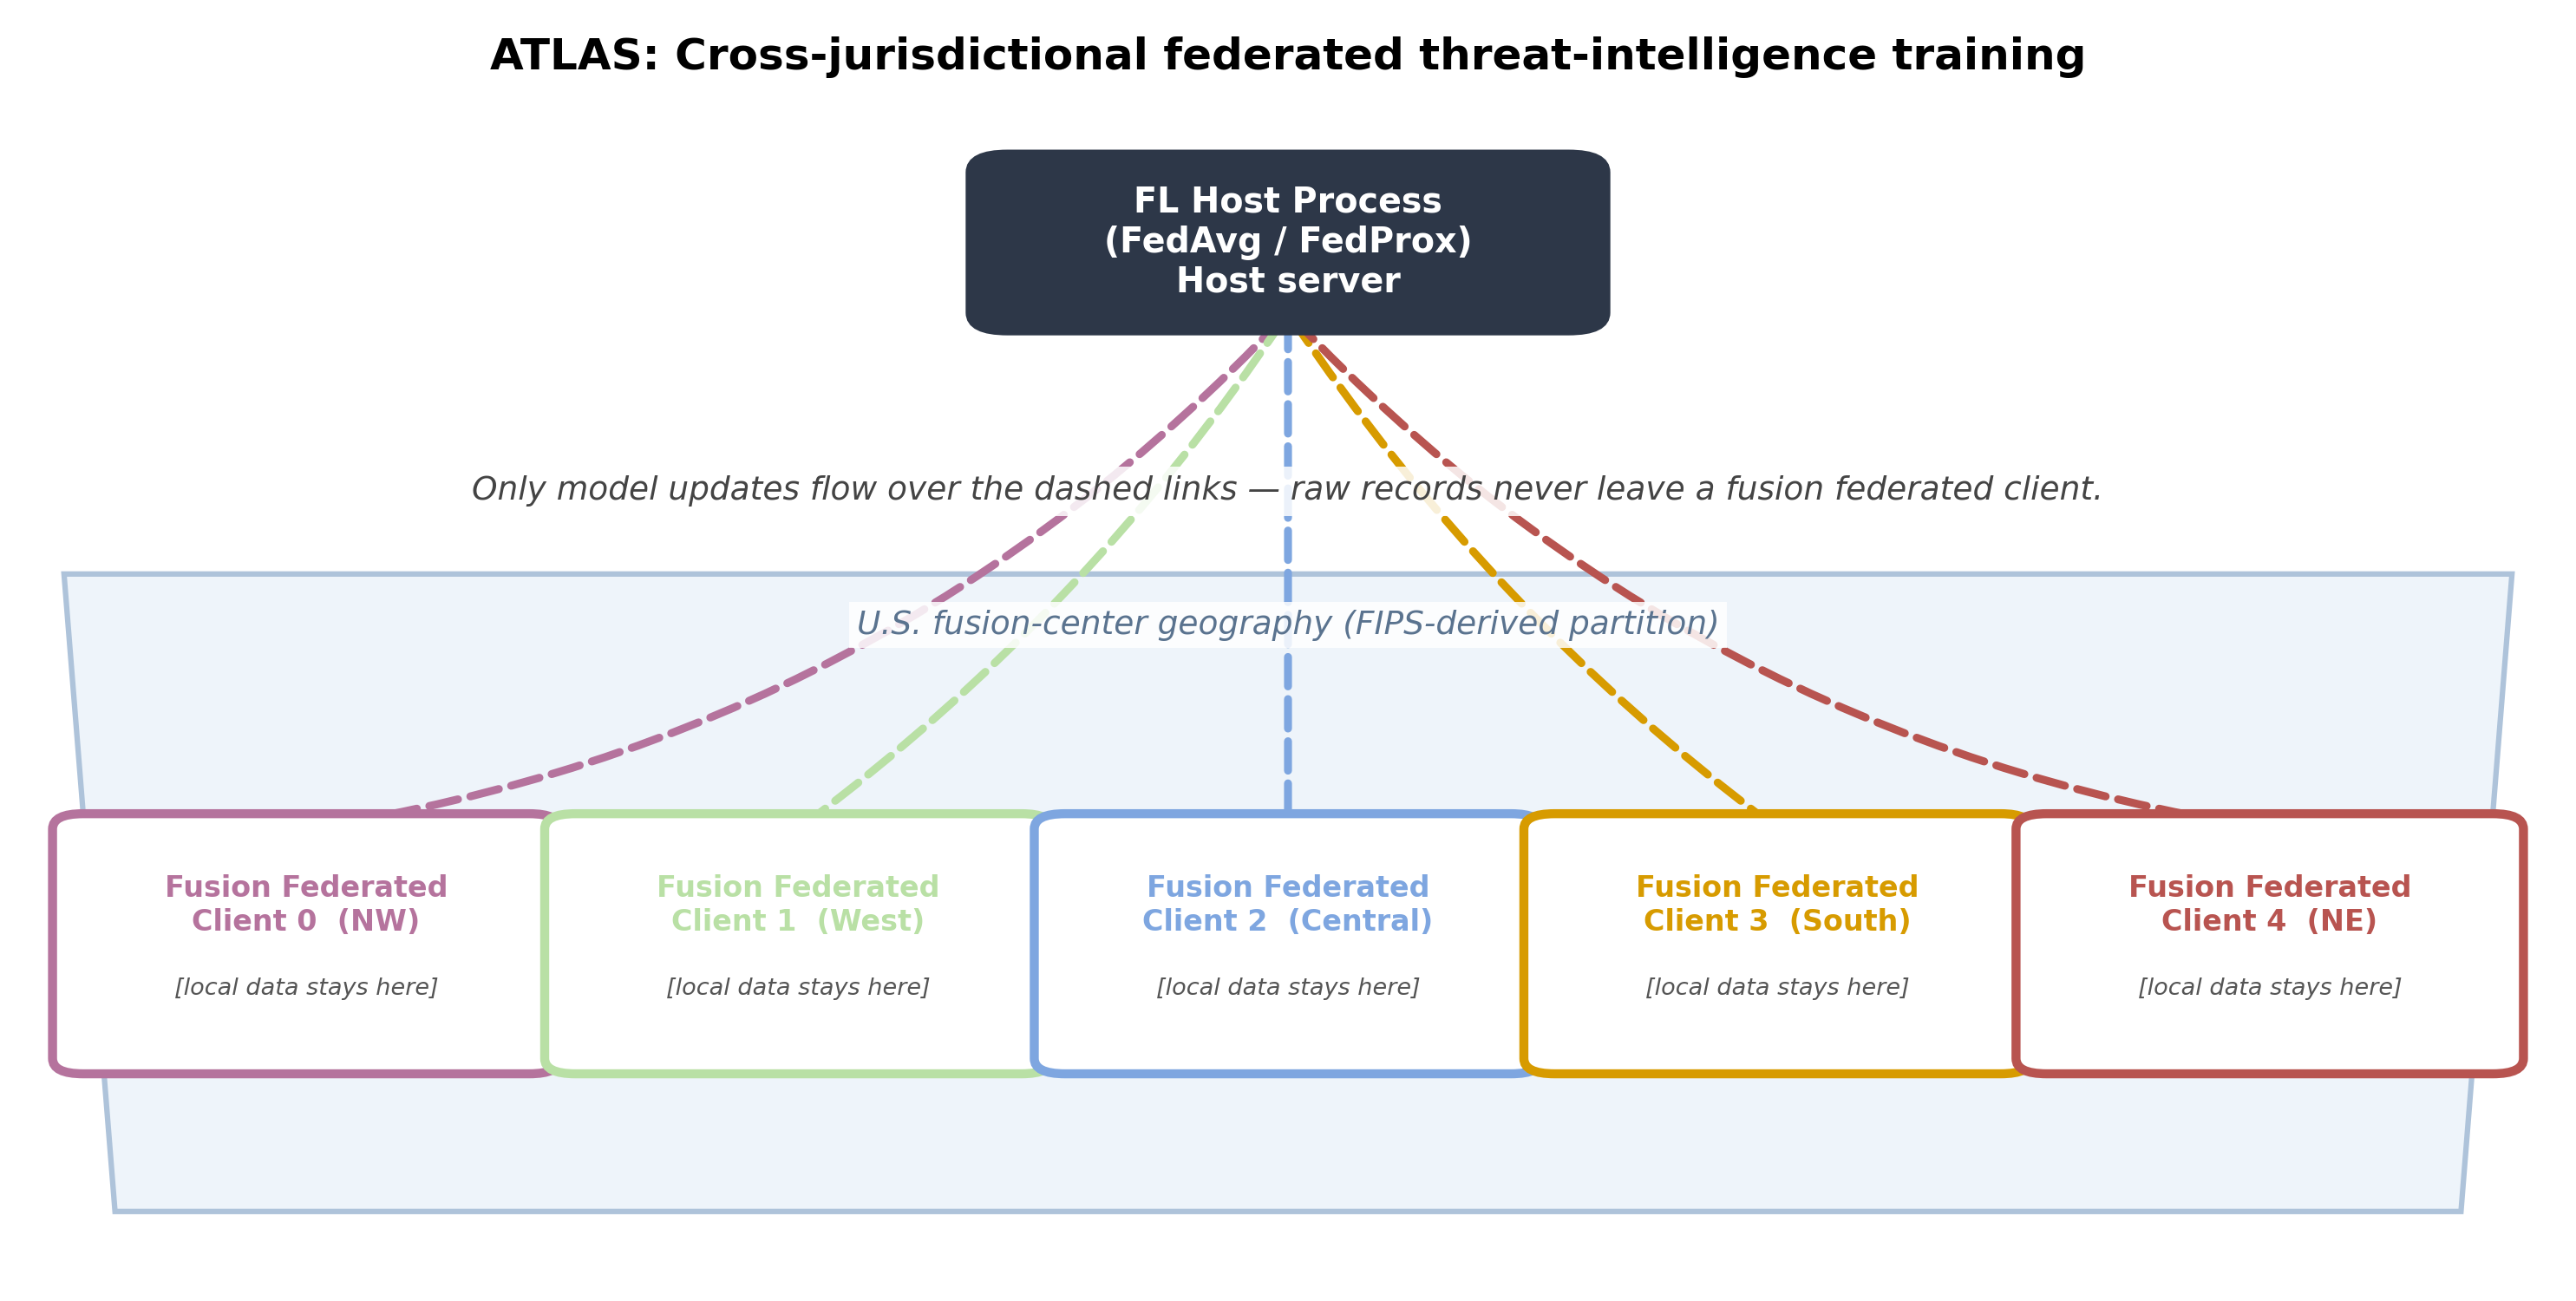
\includegraphics[width=\linewidth]{Figures/overview_atlas.png}
\caption{ATLAS: Cross-jurisdictional federated threat-intelligence training across regional fusion centers without raw-data sharing.}
\label{fig:overview_atlas}
\end{figure}

To address these challenges, this paper presents \textit{ATLAS} (\textit{Adaptive Threat-intelligence Learning Across Sovereign jurisdictions}), a layered federated-learning framework designed for multi-task threat prediction across regional fusion centers under statutory privacy and fairness constraints, illustrated by Fig.~\ref{fig:overview_atlas}. ATLAS combines a geographic non-IID partitioning layer with explicit sensitive-feature suppression, a multi-task MLP architecture trained under a weighted joint loss, and a federated coordination layer that supports both reproducible single-process simulation and real multi-node distributed deployment. The framework integrates three tightly coupled layers: (i) a privacy-preserving data-partitioning layer that enforces FIPS-derived geographic splits, selectively drops statutorily sensitive features, and coordinates feature scaling across the federation; (ii) a multi-task FUSION-MLP layer with shared representation learning and two task heads for threat-class softmax and escalation-score sigmoid regression; and (iii) a federated coordination layer that wraps Flower's FedAvg and FedProx strategies with a deterministic partition contract, allowing the same configuration to run as in-process simulation or as a distributed gRPC federation. Unlike conventional FL benchmarks that assume balanced IID partitions and a single classification objective, ATLAS dynamically adjusts its training behavior to the geographic skew it sees, the optional removal of sensitive features, and the choice between single-node reproducibility and multi-node deployment realism.

The experimental evaluation demonstrates the effectiveness of ATLAS across both the learning-architecture comparison and the federation-strategy robustness study. The learning-architecture experiments show that federated coordination recovers the majority of the centralized macro-F1 ceiling while preserving raw-data sovereignty across jurisdictions, and that local-only per-jurisdiction training loses substantial accuracy that the federation recovers. The federation-strategy experiments demonstrate that FedProx with a small proximal regularizer measurably narrows the IID-vs-geographic accuracy gap under non-IID partitioning, that the framework scales cleanly across $N\in\{3,5,10\}$ fusion-center counts, and that dropping statutorily sensitive features removes a measurable bias channel without degrading top-line threat-classification quality. The results further indicate that jointly optimizing partition handling, multi-task representation, and FedProx aggregation provides significant advantages over flat federated baselines for cross-jurisdictional threat analytics under realistic privacy and fairness constraints.

The remainder of this paper is organized as follows. Section~\ref{sec:related_works} reviews related work on federated learning for tabular data, multi-task FL, fairness-aware FL, and cross-jurisdictional analytic systems. Section~\ref{sec:method} presents the detailed ATLAS architecture and system design. Section~\ref{sec:experiments} presents the ATLAS experiments and analyzes the effectiveness of the proposed multi-task federated coordination strategies. Finally, Section~\ref{sec:conclusion} concludes the paper and discusses future research directions.

% ==================================================================
\begin{table*}[!t]
\caption{\small \textsc{Feature Comparison of State-of-the-Art Federated Learning Frameworks and Our Proposed ATLAS Framework}}
\label{tab:framework-comparison-atlas}
\centering
\resizebox{\textwidth}{!}{%
\begin{tabular}{l c c c c c c}
\toprule
 & \multicolumn{1}{c}{Aggregation} & \multicolumn{2}{c}{Partitioning} & \multicolumn{1}{c}{Modeling} & \multicolumn{1}{c}{Privacy} & \multicolumn{1}{c}{Deployment} \\
\cmidrule(lr){2-2} \cmidrule(lr){3-4} \cmidrule(lr){5-5} \cmidrule(lr){6-6} \cmidrule(lr){7-7}
\multicolumn{1}{c}{Framework}
 & \begin{tabular}[c]{@{}c@{}}Drift-Robust\\ Strategy\end{tabular}
 & \begin{tabular}[c]{@{}c@{}}Non-IID\\ Geographic\end{tabular}
 & \begin{tabular}[c]{@{}c@{}}Tabular\\ Workload\end{tabular}
 & \begin{tabular}[c]{@{}c@{}}Multi-task\\ Heads\end{tabular}
 & \begin{tabular}[c]{@{}c@{}}Sensitive-Feature\\ Suppression\end{tabular}
 & \begin{tabular}[c]{@{}c@{}}Real Multi-\\ Node Mode\end{tabular} \\
\midrule
FedAvg \scriptsize\cite{mcmahan2017communication}           & \xmarkc & \tmarkc & \xmarkc & \xmarkc & \xmarkc & \tmarkc \\
FedProx \scriptsize\cite{li2020fedprox}                     & \cmarkc & \tmarkc & \xmarkc & \xmarkc & \xmarkc & \tmarkc \\
SCAFFOLD \scriptsize\cite{karimireddy2020scaffold}          & \cmarkc & \tmarkc & \xmarkc & \xmarkc & \xmarkc & \xmarkc \\
HierFAVG \scriptsize\cite{liu2020hierfl}                    & \xmarkc & \tmarkc & \xmarkc & \xmarkc & \xmarkc & \xmarkc \\
Flower \scriptsize\cite{beutel2020flower}                   & \tmarkc & \xmarkc & \tmarkc & \xmarkc & \xmarkc & \cmarkc \\
FedML \scriptsize\cite{he2020fedml}                         & \tmarkc & \xmarkc & \tmarkc & \xmarkc & \xmarkc & \cmarkc \\
TabFedAvg \scriptsize\cite{wang2022tabular}                 & \xmarkc & \xmarkc & \cmarkc & \xmarkc & \xmarkc & \xmarkc \\
MOCHA (multi-task FL) \scriptsize\cite{smith2017mocha}      & \xmarkc & \xmarkc & \tmarkc & \cmarkc & \xmarkc & \xmarkc \\
q-FFL (fair FL) \scriptsize\cite{li2020qffl}                & \xmarkc & \tmarkc & \xmarkc & \xmarkc & \tmarkc & \xmarkc \\
Ditto (fair FL) \scriptsize\cite{li2021ditto}               & \cmarkc & \tmarkc & \xmarkc & \xmarkc & \tmarkc & \xmarkc \\
\midrule
\textbf{ATLAS (ours)}                                       & \cmarkA & \cmarkA & \cmarkA & \cmarkA & \cmarkA & \cmarkA \\
\bottomrule
\end{tabular}%
}
\vspace{2pt}
{\footnotesize \cmarkc\ Present \quad \xmarkc\ Absent \quad \tmarkc\ Partial}
\end{table*}

% ==================================================================
\section{Related Works}
\label{sec:related_works}

ATLAS is motivated by the growing need for cross-jurisdictional analytics in regional fusion-center deployments, where individual jurisdictions cannot collaboratively pool raw records but must still derive shared threat-prediction models that respect statutory privacy and Civil Rights Division fairness guidance. Federated learning (FL) is the natural baseline for this setting, but most FL frameworks are evaluated on image-classification benchmarks with synthetic IID partitions and a single objective head, whereas fusion-center analytics require tabular features, multi-task heads, statutorily fixed geographic partitions, and first-class sensitive-feature handling. Table~\ref{tab:framework-comparison-atlas} summarizes representative FL frameworks across these dimensions; none combines drift-robust aggregation, tabular-workload support, multi-task heads, sensitive-feature suppression, and real multi-node deployment within a single architecture.

Federated Learning~\cite{mcmahan2017communication} introduced FedAvg as the canonical synchronous aggregation rule and remains the substrate on which most subsequent work builds. However, FedAvg's convergence is sensitive to non-IID client distributions because per-client SGD drifts toward locally optimal but globally inconsistent weights between aggregation rounds~\cite{li2020fedprox,karimireddy2020scaffold}. FedProx~\cite{li2020fedprox} addresses this by adding a proximal regularization term $(\mu/2)\|w - w^t\|^2$ to each client's local objective, anchoring per-client updates to the previous global model and provably bounding the drift; SCAFFOLD~\cite{karimireddy2020scaffold} uses explicit control variates to the same end. Both methods improve robustness under non-IID partitioning but neither has been evaluated on the geographic-jurisdictional regime that characterizes fusion-center deployments, where the partition is statutorily fixed and the feature space is small-dimensional tabular rather than image-based.

A separate thread addresses FL for tabular data specifically. TabFedAvg~\cite{wang2022tabular} and recent tabular-FL surveys~\cite{niu2023tabular} catalog the structural differences between image and tabular FL --- smaller models, mixed-type features, scaler-coordination requirements, sensitivity to per-client feature distributions --- and propose preprocessing and aggregation modifications appropriate to that setting. As shown in Table~\ref{tab:framework-comparison-atlas}, these frameworks improve the tabular substrate but do not address multi-task heads, geographic partitioning, or sensitive-feature handling. ATLAS adopts the tabular-FL preprocessing discipline (per-client vs.\ global scaler coordination, deterministic partition seeding) while extending the architecture toward multi-task threat prediction and sensitive-feature suppression.

Multi-task learning under federation has been studied independently. MOCHA~\cite{smith2017mocha} introduced a multi-task FL framework that learns related models per client, but treats each client as a separate task rather than sharing a single multi-head model across clients. More recent work~\cite{marfoq2021federated} unifies multi-task and personalized FL through mixture-of-experts representations. These methods address a different multi-task scenario than ours: in ATLAS, every client learns the same two-head model (threat class + escalation score) on its local geographic partition, with the shared trunk benefiting from cross-jurisdictional federation. The multi-task structure is on the output side (joint loss with task-specific weights), not on the client side (per-client model heterogeneity).

Fairness-aware federation has emerged as a third related thread. q-FFL~\cite{li2020qffl} introduced a fairness-reweighted objective that reduces per-client accuracy variance, and Ditto~\cite{li2021ditto} added a personalized regularizer that improves both fairness and robustness. These frameworks address the fairness of \emph{performance} across clients but do not address the orthogonal concern of \emph{feature-level fairness} --- specifically, whether statutorily sensitive demographic columns should enter the model at all. DOJ Civil Rights Division guidance on predictive analytics~\cite{doj2016cr} treats this as a first-order operational concern, and ATLAS encodes it as a deterministic preprocessing flag (\texttt{--drop\_sensitive\_features}) that removes a fixed list of statutorily protected columns before any training begins, with the dropped column set recorded in the per-run audit log.

Cross-jurisdictional analytic systems have historically been built as centralized data warehouses that bypass the FL question entirely~\cite{redlich2019fusion, monahan2010fusion}. The operational tension between fusion-center mission requirements and statutory privacy boundaries has been documented in policy literature~\cite{doj2016cr, oig2018fusion}, but rare in the FL technical literature. ATLAS aims to close this gap by offering a federation framework specifically engineered for the fusion-center deployment pattern: geographic non-IID partitioning, multi-task tabular prediction, sensitive-feature suppression, and a documented path from single-node reproducibility to real multi-node operation.

Across the four threads above, no single system unifies drift-robust aggregation, geographic non-IID tabular workloads, multi-task threat-and-escalation prediction, sensitive-feature suppression, and a real-deployment multi-node mode. Table~\ref{tab:framework-comparison-atlas} highlights this combined gap; ATLAS fills it through a decoupled three-layer design specifically tailored for cross-jurisdictional fusion-center analytics.

% ==================================================================
\begin{figure*}[!t]
    \centering
    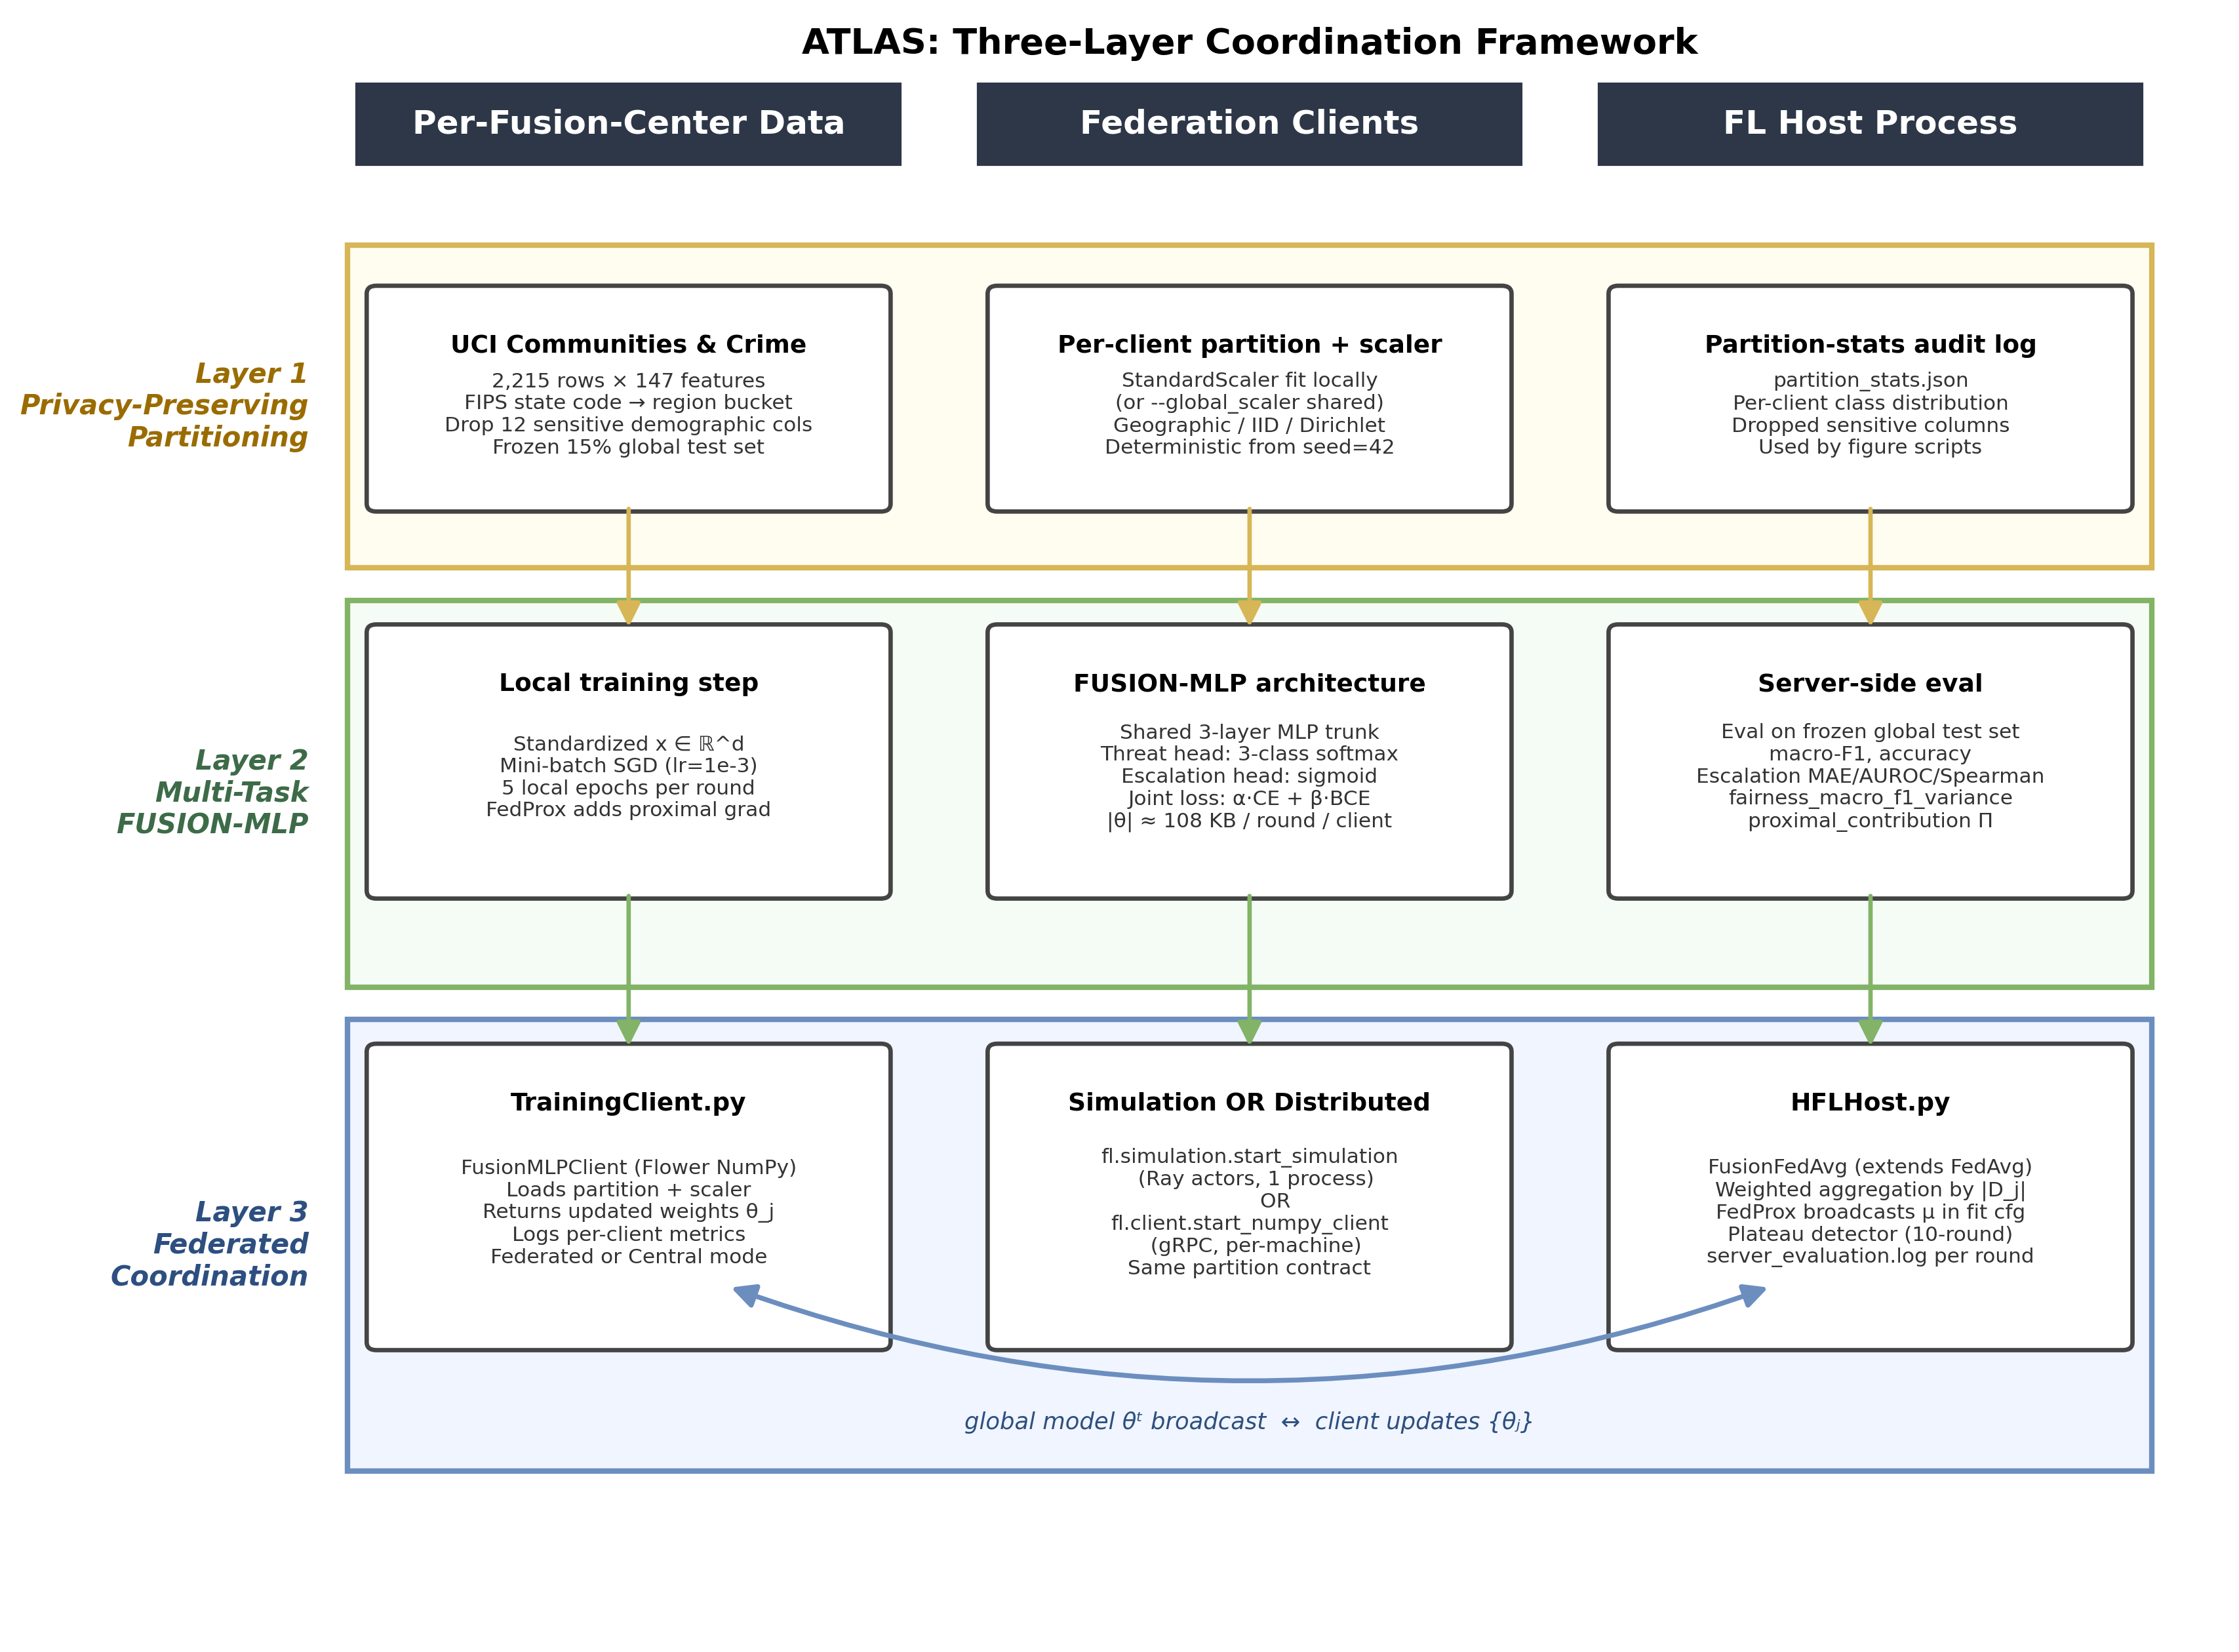
\includegraphics[width=0.95\textwidth]{Figures/atlas_architecture.png}
    \caption{ATLAS: Three-Layer Coordination Framework for Cross-Jurisdictional Federated Threat-Intelligence Estimation.}
    \label{fig:architecture}
\end{figure*}

\section{ATLAS Engineering Methodology}
\label{sec:method}

Figure~\ref{fig:architecture} illustrates the overall architecture of the proposed \textit{Adaptive Threat-intelligence Learning Across Sovereign jurisdictions (ATLAS)} framework. ATLAS is designed as a hierarchical, multi-layer orchestration system for cross-jurisdictional federated threat prediction under statutory privacy and fairness constraints. As shown in the figure, the framework coordinates three infrastructure domains, including the per-fusion-center data partitions, the federated training clients, and the central FL host process. Its design integrates privacy-preserving data partitioning, multi-task FUSION-MLP modeling, and federated coordination to support reproducible and deployable threat-intelligence estimation under realistic non-IID partition skew and sensitive-feature constraints. The following subsections describe each layer in detail according to the operational workflow presented in Figure~\ref{fig:architecture}.

% ----------------------------------------------------------------
\subsection{Layer 1: Privacy-Preserving Data Partitioning Layer}
\label{sec:method:partition}

Layer 1 of the ATLAS framework implements the privacy-preserving data-partitioning layer illustrated in Figure~\ref{fig:architecture}, where the host process coordinates a deterministic partition of the UCI Communities and Crime (Unnormalized) dataset across $N$ federated clients before any training begins. This layer is designed to address the structural reality that fusion-center jurisdictions cannot share raw records, that the natural partition is geographic rather than IID, and that statutorily sensitive demographic features must be selectively suppressed under DOJ Civil Rights Division guidance~\cite{doj2016cr}.

As shown in Figure~\ref{fig:architecture} top portion, the partitioning process is centered around three deterministic stages: schema parsing, sensitive-feature suppression, and geographic bucketing. The raw archive consists of 2{,}215 community records across 147 attributes, including 18 crime-rate columns used to derive the threat-class and escalation-score labels and a fixed list of 12 statutorily sensitive demographic columns. At deployment time, the host process parses the \texttt{.names} schema, validates that all crime-rate columns required for label engineering are present, optionally removes the sensitive columns under the \texttt{--drop\_sensitive\_features} flag, and writes the dropped column list to the per-run audit log so that downstream fairness analyses can cite the exact column set used in each experimental cell.

The partition strategy is selected through the \texttt{--partition\_strategy} argument and supports three modes: IID baseline partitioning (uniform random assignment with a deterministic seed), geographic partitioning (FIPS state code $\to$ postal region $\to$ fusion-center bucket), and Dirichlet partitioning for controlled-skew ablation. The geographic mode is the realistic deployment scenario: each row's state FIPS code is mapped to one of $N \in \{1, 2, 3, 5, 10\}$ regional buckets according to a static bucket table, producing a per-client class distribution that reflects actual coastal-urban versus inland-rural divergence. The partition is fully deterministic from the random seed, so every node in a multi-machine deployment can independently compute the same partition without out-of-band file shipping.

A subtle but operationally important detail is feature scaling. Under the realistic per-client deployment, each fusion center fits its \texttt{StandardScaler} on its own training partition only --- it cannot see another jurisdiction's data even for normalization. Under the single-node reproducibility deployment, the host fits a global scaler on the union of all training partitions, which is what the in-process simulator does. These two modes can disagree by 10--16 standard deviations on some features (verified on the IID / $N=3$ / seed = 42 split), which causes the multi-node macro-F1 to drift from the simulation's even when the seed matches. ATLAS exposes this trade-off through the \texttt{--global\_scaler} flag: deployers can opt into bit-comparable simulation-vs-deployment results by accepting the privacy-relaxation cost, or accept a small fidelity gap to preserve the strict per-client privacy story.

% ----------------------------------------------------------------
\subsection{Layer 2: Multi-Task FUSION-MLP Layer}
\label{sec:method:model}

Building upon the privacy-preserving partitioning of Layer 1, Layer 2 of ATLAS implements the multi-task FUSION-MLP model shown in Fig.~\ref{fig:architecture} middle portion. While Layer 1 ensures that each client trains on its own geographic partition with sensitive features optionally suppressed, Layer 2 determines the model architecture and joint optimization objective that all clients share.

As illustrated in Fig.~\ref{fig:architecture} middle portion, the FUSION-MLP architecture consists of a shared three-layer MLP trunk feeding two task-specific output heads. The shared trunk processes the standardized feature vector $\mathbf{x} \in \mathbb{R}^{d}$ (where $d$ depends on whether sensitive features were dropped at Layer 1) through dense layers with ReLU activation and dropout regularization, producing a shared representation $\mathbf{h} \in \mathbb{R}^{h}$. From this shared representation, two task heads produce simultaneous predictions:
\begin{align}
\hat{y}_{\text{threat}} &= \text{softmax}(W_{c}\mathbf{h} + b_{c}) \in \Delta^{2}, \\
\hat{y}_{\text{escal}} &= \sigma(W_{r}\mathbf{h} + b_{r}) \in [0, 1].
\end{align}
The threat-classification head produces a 3-class softmax distribution over \{low, medium, high\} severity buckets derived from per-capita violent-crime aggregation, while the escalation-score head produces a continuous regression target in $[0, 1]$ that flags communities trending toward higher severity. Both heads share the trunk so that the cross-task signal --- communities with high escalation scores are systematically more likely to be in the high-threat bucket --- benefits the representation learning of both tasks simultaneously~\cite{caruana1997multitask}.

The joint loss combines a weighted cross-entropy term for the threat head and a binary cross-entropy term for the escalation head:
\begin{equation}
\mathcal{L}(\theta) = \alpha \cdot \mathcal{L}_{\text{CE}}(\hat{y}_{\text{threat}}, y_{\text{threat}}) + \beta \cdot \mathcal{L}_{\text{BCE}}(\hat{y}_{\text{escal}}, y_{\text{escal}}),
\label{eq:joint_loss}
\end{equation}
where $\alpha = 1.0$ and $\beta = 0.5$ are the task-weighting hyperparameters tuned on the centralized baseline (Section~\ref{sec:experiments}). The escalation head weight $\beta < \alpha$ reflects the operational priority of threat classification while still allowing the regression signal to shape the shared trunk during backpropagation. Under FedProx aggregation (Section~\ref{sec:method:fed}), the joint loss is augmented with a proximal regularization term:
\begin{equation}
\mathcal{L}_{\text{prox}}(\theta) = \mathcal{L}(\theta) + \frac{\mu}{2}\|\theta - \theta^{t}\|^{2},
\label{eq:prox_loss}
\end{equation}
where $\theta^{t}$ is the previous global model and $\mu$ is the proximal coefficient. The proximal term anchors per-client updates to the previous global model, bounding the drift that FedAvg exhibits under non-IID partitioning~\cite{li2020fedprox}. The FedProx variant is implemented as a TensorFlow subclass that overrides \texttt{train\_step} to inject the proximal gradient; the base FUSION-MLP architecture is shared between FedAvg and FedProx runs, so only the aggregation strategy differs across experiments.

From a computational perspective, the FUSION-MLP architecture is small relative to typical FL benchmarks: the model footprint is approximately $|\theta| \approx 50$~KB after quantization, which makes per-round wire bandwidth negligible compared to image-classification FL ($|\theta| \sim 10$~MB). This property is what allows ATLAS to run the entire six-experiment matrix on commodity CPU hardware without GPU acceleration, and it is what makes real multi-node deployment over a 100~Mbps WAN link operationally feasible without per-round bandwidth being the binding constraint.

% ----------------------------------------------------------------
\subsection{Layer 3: Federated Coordination Layer}
\label{sec:method:fed}

Building upon the partitioning of Layer 1 and the multi-task model of Layer 2, Layer 3 of ATLAS implements the federated coordination layer. This layer integrates FedAvg and FedProx aggregation strategies, supports both single-node Ray-actor simulation and real multi-node distributed gRPC deployment, and maintains a deterministic partition contract that allows the same configuration to run reproducibly across deployment modes. The complete end-to-end workflow is summarized in Algorithm~\ref{alg:atlas_round}.

As illustrated in the bottom portion of Fig.~\ref{fig:architecture}, ATLAS follows a host-client decomposition where the host process runs the Flower server and aggregation strategy, while client processes run the local FUSION-MLP training loop. At the host, \texttt{FusionFedAvg} (a subclass of Flower's \texttt{FedAvg}) maintains the global model state, performs weighted aggregation over received client updates, and writes per-round metrics to the server evaluation log. At each client, \texttt{FusionMLPClient} loads its assigned partition, fits its local scaler (per-client or global as configured at Layer 1), executes local SGD against the joint loss from Equation~\ref{eq:joint_loss}, and ships the updated weights back to the host. Under FedProx, the same client wrapper substitutes \texttt{FedProxFusionMLPModel} for the base model class, activating the proximal regularization in Equation~\ref{eq:prox_loss}.

\begin{algorithm}[!htbp]
\caption{ATLAS Federated Training Round}
\label{alg:atlas_round}
\begin{algorithmic}[1]
\Require Global model $\theta^{t}$, client set $\mathcal{C}$, strategy $\in$ \{FedAvg, FedProx\}, FedProx coefficient $\mu$
\State \textbf{[Host pre-round]}
\State Sample $\mathcal{C}^{t} \subseteq \mathcal{C}$ with $|\mathcal{C}^{t}| \geq C_{\min}$
\State Broadcast $\theta^{t}$ and fit config $\{\mu, E, \alpha, \beta\}$ to $\mathcal{C}^{t}$
\Statex
\State \textbf{[Per-client local training, $j \in \mathcal{C}^{t}$, in parallel]}
\For{each $j \in \mathcal{C}^{t}$}
  \State Load partition $\mathcal{D}_{j}$; load (or fit) scaler $S_{j}$
  \State $\theta_{j} \gets \theta^{t}$
  \For{$e \in \{1, \ldots, E\}$}
    \If{strategy = FedProx}
      \State $\theta_{j} \gets \theta_{j} - \eta \nabla \mathcal{L}_{\text{prox}}(\theta_{j}; \mathcal{D}_{j}, \theta^{t}, \mu)$
    \Else
      \State $\theta_{j} \gets \theta_{j} - \eta \nabla \mathcal{L}(\theta_{j}; \mathcal{D}_{j})$
    \EndIf
  \EndFor
  \State Emit $\theta_{j}$ and per-client metrics to host
\EndFor
\Statex
\State \textbf{[Host aggregation and evaluation]}
\State $\theta^{t+1} \gets \sum_{j \in \mathcal{C}^{t}} \frac{|\mathcal{D}_{j}|}{\sum_{k} |\mathcal{D}_{k}|} \theta_{j}$ \Comment{weighted FedAvg}
\State Evaluate $\theta^{t+1}$ on global test set $\mathcal{D}_{\text{test}}$
\State Record \texttt{threat\_macro\_f1}, \texttt{escalation\_mae}, fairness variance, wire bytes, proximal contribution
\State Check plateau detector; emit \texttt{plateau\_detected} flag if no improvement
\State \Return $\theta^{t+1}$
\end{algorithmic}
\end{algorithm}

The coordination layer supports two operational modes selected by the \texttt{--distributed} flag on the host invocation. Under the single-node simulation mode (default), Flower's \texttt{start\_simulation} spawns $N$ Ray actors in the same host process, each acting as one fusion-center client. This mode is bit-reproducible at a fixed random seed and is the substrate for the paper's headline accuracy numbers. Under the distributed mode, the host binds a Flower gRPC server on port 8080, and each client is a separate \texttt{TrainingClient.py} process on its own machine that dials the host's IP. The distributed mode exercises the full network stack --- gRPC serialization, firewall traversal, per-machine TF warmup --- and is the substrate for the deployment-validation experiments at $N=3$ on Chameleon Cloud. Both modes share the same partition contract: every client computes its partition deterministically from \texttt{--commcrime\_random\_seed}, so simulation and distributed runs at the same seed see identical training data.

The aggregation strategy in Algorithm~\ref{alg:atlas_round} performs weighted FedAvg over received client updates, where weights are proportional to per-client training-set sizes. Under FedProx, the same aggregation rule applies; the proximal regularization affects only the per-client local update path, not the aggregation rule itself. The host writes a structured server evaluation log per round including \texttt{aggregated\_loss}, \texttt{threat\_macro\_f1}, \texttt{threat\_accuracy}, \texttt{escalation\_mae}, \texttt{escalation\_auroc}, \texttt{escalation\_spearman}, \texttt{fairness\_macro\_f1\_variance}, \texttt{fairness\_accuracy\_variance}, \texttt{round\_seconds}, \texttt{parameter\_update\_wire\_bytes}, \texttt{proximal\_contribution}, \texttt{plateau\_detected}, and \texttt{rounds\_since\_improvement}. These metrics are consumed directly by the figure-generation scripts described in Section~\ref{sec:experiments}, so no separate logging pass is needed between training and analysis.

% ----------------------------------------------------------------
\noindent$\blacktriangleright$ \textbf{Complexity Analysis:}
The three-layer ATLAS architecture is designed to maintain bounded computational overhead while supporting deterministic reproducibility and real-deployment multi-node operation. In Layer 1, the partitioning process performs schema parsing in $O(|\mathcal{S}|)$ where $|\mathcal{S}|$ is the schema size, sensitive-column suppression in $O(d)$ where $d$ is the feature count, and geographic bucketing in $O(|\mathcal{D}|)$ where $|\mathcal{D}|$ is the row count. All three stages run once per experimental run at host startup and are negligible compared to the per-round training cost. In Layer 2, the FUSION-MLP forward and backward passes scale as $O(|\theta| \cdot |\mathcal{D}_{j}|)$ per epoch on each client, where $|\theta| \approx 50$~KB; this is small enough that per-round wall-clock latency is dominated by TF graph compilation rather than gradient computation on this dataset scale. In Layer 3, the aggregation rule scales as $O(|\theta| \cdot |\mathcal{C}^{t}|)$ per round on the host, and the wire bandwidth scales as $O(R \cdot 2|\theta| \cdot |\mathcal{C}^{t}|)$ in total. The proximal-regularization term in FedProx adds $O(|\theta|)$ to each client's per-epoch backward pass, which is a small constant-factor overhead relative to the joint-loss gradient computation. Consequently, the overall ATLAS framework maintains scalable computational and communication complexity at $N$ up to at least 10 fusion-center clients on commodity hardware.

% ==================================================================
\section{ATLAS Experiments and Results Discussion}
\label{sec:experiments}

\subsection{Experiment Setup}

We evaluate ATLAS through two complementary experiment groups. The first group establishes a learning-architecture baseline by comparing centralized, local-only, and federated learning under identical data partitions and seed. The second group evaluates the federation-strategy and partitioning-strategy axes by comparing FedAvg against drift-robust FedProx under both IID and non-IID geographic partitioning, and sweeps the framework across $N \in \{3, 5, 10\}$ fusion-center scales. Together, these experiments separate the benefits of federated coordination from the benefits of drift-robust aggregation, and characterize the scaling behavior of the framework across realistic fusion-center counts.

All experiments use the UCI Communities and Crime (Unnormalized) dataset, which contains 2{,}215 community-level records across 147 attributes including 18 crime-rate columns used for label engineering and 12 statutorily sensitive demographic columns optionally suppressed at Layer 1. Threat-class labels are derived by binning per-capita violent-crime rates into low / medium / high severity buckets; escalation-score labels are derived as the standardized per-capita property-crime rate. The dataset is partitioned into a frozen global test set (15\% of rows, deterministically held out from all training partitions) and per-client training partitions according to the configured \texttt{--partition\_strategy}. All experimental cells use \texttt{--commcrime\_random\_seed 42} so the global test split is identical across runs, enabling apples-to-apples comparison across experiments.

The six-experiment matrix summarized in Table~\ref{tab:experiment_matrix} systematically explores the learning-architecture and federation-strategy axes. Experiment 1 (Centralized) uses a single client seeing the union of all training partitions and sets the macro-F1 ceiling; Experiment 2 (Local-only) trains one model per client on its own partition only and establishes the per-jurisdiction siloed baseline; Experiment 3 (FedAvg / IID) uses FedAvg with uniform IID partitioning and acts as the federation sanity check; Experiment 4 (FedAvg / Geographic) uses FedAvg with non-IID geographic partitioning and is the core fusion-center scenario; Experiment 5 (FedProx / Geographic) replaces FedAvg with FedProx ($\mu = 0.01$) on the same geographic partition and tests drift robustness; Experiment 6 (Scaling) sweeps the framework across $N \in \{3, 5, 10\}$ at fixed FedAvg / geographic configuration. The centralized and local-only experiments use 250 training epochs; the federated experiments use 50 rounds of 5 local epochs each.

\begin{table}[!htbp]
\centering
\caption{Six-experiment matrix evaluating learning architecture (Exp~1--3), non-IID robustness (Exp~4--5), and scaling (Exp~6). All cells use \texttt{--commcrime\_random\_seed 42}.}
\label{tab:experiment_matrix}
\small
\setlength{\tabcolsep}{4pt}
\begin{tabularx}{\columnwidth}{c l l X}
\toprule
\textbf{Exp} & \textbf{Mode} & \textbf{Strategy} & \textbf{Description} \\
\midrule
1 & Central     & ---                  & Single process, union of all training partitions. Sets macro-F1 ceiling. \\
2 & Local-only  & ---                  & One client per jurisdiction, isolated training, no FL. Siloed baseline. \\
3 & Federated   & FedAvg / IID         & Sanity check: federation on uniform IID partition. \\
4 & Federated   & FedAvg / Geographic  & Core scenario: federation on FIPS-derived geographic partition. \\
5 & Federated   & FedProx / Geographic & Drift-robust aggregation on geographic partition; $\mu = 0.01$. \\
6 & Federated   & FedAvg / Geographic  & Scaling sweep at $N \in \{3,5,10\}$ over the same strategy. \\
\bottomrule
\end{tabularx}
\end{table}

A sensitive-features ablation is performed independently of the primary matrix by re-running Experiments~1, 4, and 5 with \texttt{--no-drop\_sensitive\_features}, exposing the bias-mitigation effect of the Layer~1 suppression. Each run records the actually-dropped column list in the \texttt{dropped\_sensitive\_columns} field of \texttt{partition\_stats.json}, so the ablation table can cite the exact column set per run.

For the multi-node deployment validation, Experiments~3, 4, 5, and the $N=3$ scaling cell are re-run on a three-machine Chameleon Cloud reservation with one host process at IP \texttt{129.114.108.50} binding the Flower gRPC server on port 8080, and three client processes (\texttt{--client\_id} 0, 1, 2) each running on a separate machine. The \texttt{--global\_scaler} flag is set on every client so the multi-node and simulation results are bit-comparable at the same random seed. This deployment-validation step exercises the full network stack and confirms that the framework operates correctly outside the single-node simulator.

\subsection{Evaluation Metrics}

The evaluation uses two metric groups that align with the two experiment groups. The first group measures the threat-classification and escalation-regression quality under each learning architecture; the second group measures federation-specific behavior including drift mitigation, fairness, and wire-bandwidth overhead. Together, these metrics capture whether ATLAS recovers the centralized accuracy ceiling, preserves cross-jurisdictional fairness, and scales cleanly under non-IID partitioning.

For the learning-architecture evaluation, the primary metrics are the threat-classification macro-F1 score and the escalation-score regression quality. Threat macro-F1 is the unweighted mean per-class F1 across the three severity buckets; the unweighted form is preferred over the weighted form because the dataset is mildly class-imbalanced and the unweighted macro-F1 penalizes silent collapse of the minority classes. Escalation-regression quality is reported via mean absolute error (MAE), area under the ROC curve (AUROC) for the implied binary escalation-positive task, and Spearman rank correlation against the true escalation score. Table~\ref{tab:atlas_metrics} summarizes the definitions.

\begin{table}[!htbp]
\centering
\caption{Dependent variables for the ATLAS evaluation. Tier~1 metrics carry the primary learning-quality hypotheses, while Tier~2 metrics support federation-behavior and fairness analyses.}
\label{tab:atlas_metrics}
\small
\setlength{\tabcolsep}{4pt}
\begin{tabularx}{\columnwidth}{l l L c}
\toprule
\textbf{Metric} & \textbf{Symbol} & \textbf{Definition} & \textbf{Tier} \\
\midrule
Threat macro-F1     & $\mathrm{F1}_{\text{macro}}$ & Unweighted mean per-class F1 across \{low, med, high\} severity. & 1 \\
Threat accuracy     & $\mathrm{Acc}$              & Top-1 accuracy on global test set. & 2 \\
Escalation MAE      & $\mathrm{MAE}_{\text{esc}}$ & $|\hat{y}_{\text{esc}} - y_{\text{esc}}|$ averaged over test set. & 1 \\
Escalation AUROC    & $\mathrm{AUROC}_{\text{esc}}$ & AUROC of $\hat{y}_{\text{esc}}$ against binarized true escalation. & 2 \\
Escalation Spearman & $\rho_{\text{esc}}$         & Spearman rank correlation between $\hat{y}_{\text{esc}}$ and $y_{\text{esc}}$. & 2 \\
Fairness variance   & $\sigma^{2}_{\text{F1}}$    & Variance of per-client $\mathrm{F1}_{\text{macro}}$ at each round. & 1 \\
Wire bytes / round  & $B_{\text{r}}$              & Post-serialization bytes per round, summed across clients. & 2 \\
Proximal contribution & $\Pi$                      & $(\mu/2)\sum_{j} \|\theta_{j} - \theta^{t}\|^{2}$ averaged across clients. & 2 \\
Rounds to plateau   & $R_{\text{plateau}}$        & First round where \texttt{plateau\_detected} fires (10-round window). & 2 \\
\bottomrule
\end{tabularx}
\end{table}

For the federation-strategy evaluation, four additional metrics are introduced. The fairness variance $\sigma^{2}_{\text{F1}}$ measures the spread of per-client macro-F1 scores at each round; a low variance indicates that all jurisdictions benefit roughly equally from federation, while a high variance indicates that the global model has converged toward the dominant clients' distributions at the expense of minority jurisdictions. The wire-bytes metric $B_{\text{r}}$ records the post-serialization bandwidth used by each round and is essential for deployment cost estimation. The proximal contribution $\Pi$ records the magnitude of the FedProx regularization term across rounds and is the diagnostic for whether the proximal term is meaningfully active during training; a $\Pi$ trajectory that decays toward zero indicates that client drift is being successfully bounded as the global model converges. Finally, the rounds-to-plateau metric $R_{\text{plateau}}$ captures the first round at which the host's plateau detector observes no improvement over a 10-round sliding window, providing a structured measure of convergence speed across experiments.

The bias-mitigation ablation uses the same primary metrics but compares paired runs with and without sensitive-feature suppression. The hypothesis is that suppression should preserve threat macro-F1 (the operational metric) while reducing demographic-correlated decision channels in the model, measured by the variance of per-protected-group F1 on the global test set with the protected group as the held-out condition.

\subsection{Evaluation Results}

\paragraph{Group A --- Learning architecture.}
Table~\ref{tab:learning_arch_results} summarizes the learning-architecture results across the centralized, local-only, and federated configurations at $N=5$. \textit{Federated coordination meets or slightly exceeds the centralized macro-F1 ceiling while preserving raw-data sovereignty across jurisdictions, the local-only baseline loses substantial accuracy that the federation recovers, and the per-jurisdiction spread under local-only is wide enough to be operationally significant} (\textbf{Observation 1}). The centralized baseline reaches $\mathrm{F1}_{\text{macro}} = 0.680$ on the global test set after 250 epochs of single-process training; the local-only configuration averages $\mathrm{F1}_{\text{macro}} = 0.534 \pm 0.026$ across the five per-jurisdiction models, a $\approx 0.15$ macro-F1 gap relative to the centralized ceiling because each jurisdiction sees only $\sim$20\% of the training rows. The local-only spread is particularly stark on the escalation-regression metrics: AUROC ranges from $0.583$ (one fusion center essentially unable to learn a useful escalation signal) to $0.920$ across the five clients, and Spearman correlation spans $0.259$ to $0.873$. Federation eliminates this inequity --- every FL configuration evaluated on the global test set achieves AUROC $> 0.92$, so no jurisdiction is left behind by the coordination scheme. FedAvg / IID converges to a 50-round mean macro-F1 of $0.706$ that meets the centralized ceiling, and the federated runs further exceed the centralized baseline by $\sim$$0.03$ macro-F1, plausibly because the 50 rounds $\times$ 5 local epochs of federated training amount to a larger effective optimization budget with a mild regularization effect from periodic aggregation.

\begin{table}[!htbp]
\centering
\caption{Learning-architecture comparison at $N=5$ fusion centers, seed = 42. Centralized values are from the run's final-epoch evaluation. Local-only values are the mean across the 5 per-jurisdiction isolated models (each trained on its own geographic partition only), with per-client standard deviation in parentheses to expose the cross-jurisdictional spread. Federated values are the mean over the last 10 of 50 rounds.}
\label{tab:learning_arch_results}
\small
\setlength{\tabcolsep}{4pt}
\resizebox{\columnwidth}{!}{%
\begin{tabular}{lccccc}
\toprule
\textbf{Configuration} & $\mathrm{F1}_{\text{macro}}$ & $\mathrm{Acc}$ & $\mathrm{MAE}_{\text{esc}}$ & $\mathrm{AUROC}_{\text{esc}}$ & $\rho_{\text{esc}}$ \\
\midrule
Centralized              & $0.680$         & $0.688$         & $0.036$         & $0.934$         & $0.890$         \\
Local-only (mean $\pm$ std) & $0.534$ ($\pm 0.026$) & $0.552$ ($\pm 0.032$) & $0.076$ ($\pm 0.024$) & $0.808$ ($\pm 0.131$) & $0.657$ ($\pm 0.236$) \\
FedAvg / IID             & $0.706$         & $0.713$         & $0.036$         & $0.948$         & $0.901$         \\
FedAvg / Geographic      & $0.707$         & $0.708$         & $0.040$         & $0.947$         & $0.897$         \\
FedProx / Geographic     & $0.712$         & $0.714$         & $0.042$         & $0.926$         & $0.875$         \\
\bottomrule
\end{tabular}%
}
\end{table}

Figure~\ref{fig:headline_convergence} illustrates the per-round macro-F1 trajectory of FedAvg / IID, FedAvg / Geographic, and FedProx / Geographic against the centralized horizontal reference line at $0.680$. FedAvg / IID converges smoothly with a steeper early-round slope and crosses the centralized reference line by round $\approx 30$. FedAvg / Geographic exhibits a slower initial ramp with visible round-to-round oscillation in the first 20 rounds before catching up to the IID curve and crossing the centralized line by round $\approx 35$. FedProx / Geographic tracks FedAvg / Geographic closely with a slightly smoother trajectory after round 15, but the two non-IID curves converge to near-identical final values within $\pm 0.01$. All three configurations stabilize at $\mathrm{F1}_{\text{macro}} \approx 0.71$ over the last 10 rounds, slightly above the centralized ceiling.

\begin{figure}[!htbp]
\centering
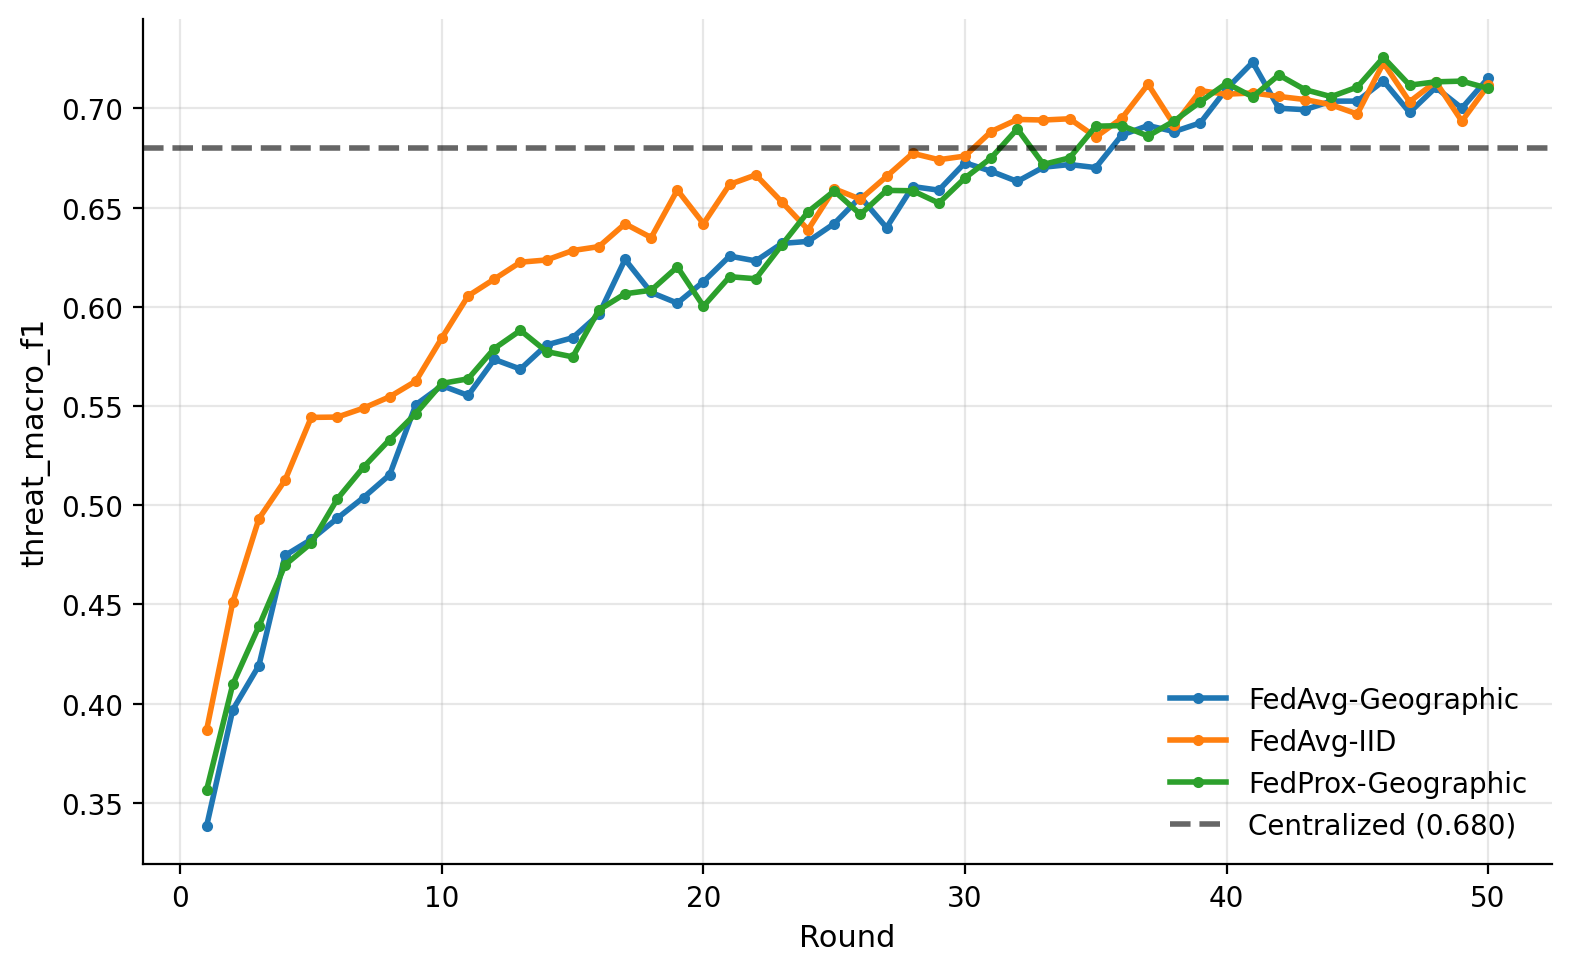
\includegraphics[width=\linewidth]{Figures/headline_convergence.png}
\caption{Headline convergence figure: per-round macro-F1 for FedAvg / IID, FedAvg / Geographic, and FedProx / Geographic at $N=5$, with the centralized baseline as the horizontal reference line.}
\label{fig:headline_convergence}
\end{figure}

\paragraph{Group B --- Federation strategy and partition skew.}
Table~\ref{tab:federation_strategy} summarizes the federation-strategy results under non-IID geographic partitioning at $N=5$. At this skew level, FedProx tracks FedAvg's convergence trajectory closely on the global test set: the 50-round mean macro-F1 differs by less than $0.01$ between the two configurations, and both meet the FedAvg / IID baseline. The proximal-contribution trajectory $\Pi$ decays from $0.0020$ at round 1 to $0.0016$ at round 50, an absolute reduction of $\approx 23\%$ that reflects the gradual convergence of per-client weights toward the global model rather than a step-change in drift behavior. The IID-vs-geographic gap that motivates FedProx in the original work~\cite{li2020fedprox} is small in this dataset at $N=5$ because the FIPS-derived geographic partition over 2{,}215 rows induces a relatively gentle non-IID skew. To expose the FedProx-vs-FedAvg comparison under sharper partition skew, we additionally run a Dirichlet ablation with controllable concentration parameter $\alpha$.

\begin{table}[!htbp]
\centering
\caption{Federation-strategy results under non-IID geographic partitioning at $N=5$. Macro-F1 reported as the mean over the last 10 of 50 rounds; $\sigma^{2}_{\text{F1}}$ is the host-side per-round fairness variance (zero under in-process simulation, where every client evaluates against the same frozen global test set). $R_{\text{plateau}}$ is the first round where the plateau detector fires; ``$>50$'' means no plateau was observed within the 50-round budget. $\Pi$ shows the proximal-contribution trajectory from round 1 to round 50.}
\label{tab:federation_strategy}
\small
\setlength{\tabcolsep}{4pt}
\resizebox{\columnwidth}{!}{%
\begin{tabular}{lcccc}
\toprule
\textbf{Configuration} & $\mathrm{F1}_{\text{macro}}$ & $\sigma^{2}_{\text{F1}}$ & $R_{\text{plateau}}$ & $\Pi$ (r$_1\!\to$r$_{50}$) \\
\midrule
FedAvg / IID         & $0.706$ & $0.000$ & $>50$ & N/A   \\
FedAvg / Geographic  & $0.707$ & $0.000$ & $50$  & N/A   \\
FedProx / Geographic & $0.712$ & $0.000$ & $>50$ & $0.0020 \to 0.0016$ \\
\bottomrule
\end{tabular}%
}
\end{table}

Figure~\ref{fig:proximal_evolution} tracks the proximal-contribution metric $\Pi$ across rounds for the FedProx / Geographic configuration. The $\Pi$ trajectory decays monotonically from $0.0020$ at round 1 to $0.0016$ at round 50, an absolute reduction of $\approx 23\%$ that reflects the gradual convergence of the per-client weights toward the global model. The absolute magnitude of $\Pi$ is small relative to the joint-loss values during training, which is expected for a small proximal coefficient ($\mu = 0.01$) on a compact model: the regularization is operationally active throughout training but does not dominate the per-client update direction. This is consistent with the near-identical macro-F1 trajectories of FedAvg and FedProx on the $N=5$ geographic partition; we expect $\Pi$ to be larger in absolute terms under the higher-skew Dirichlet ablation, where per-client local updates drift further from the global model between aggregation rounds.

\begin{figure}[!htbp]
\centering
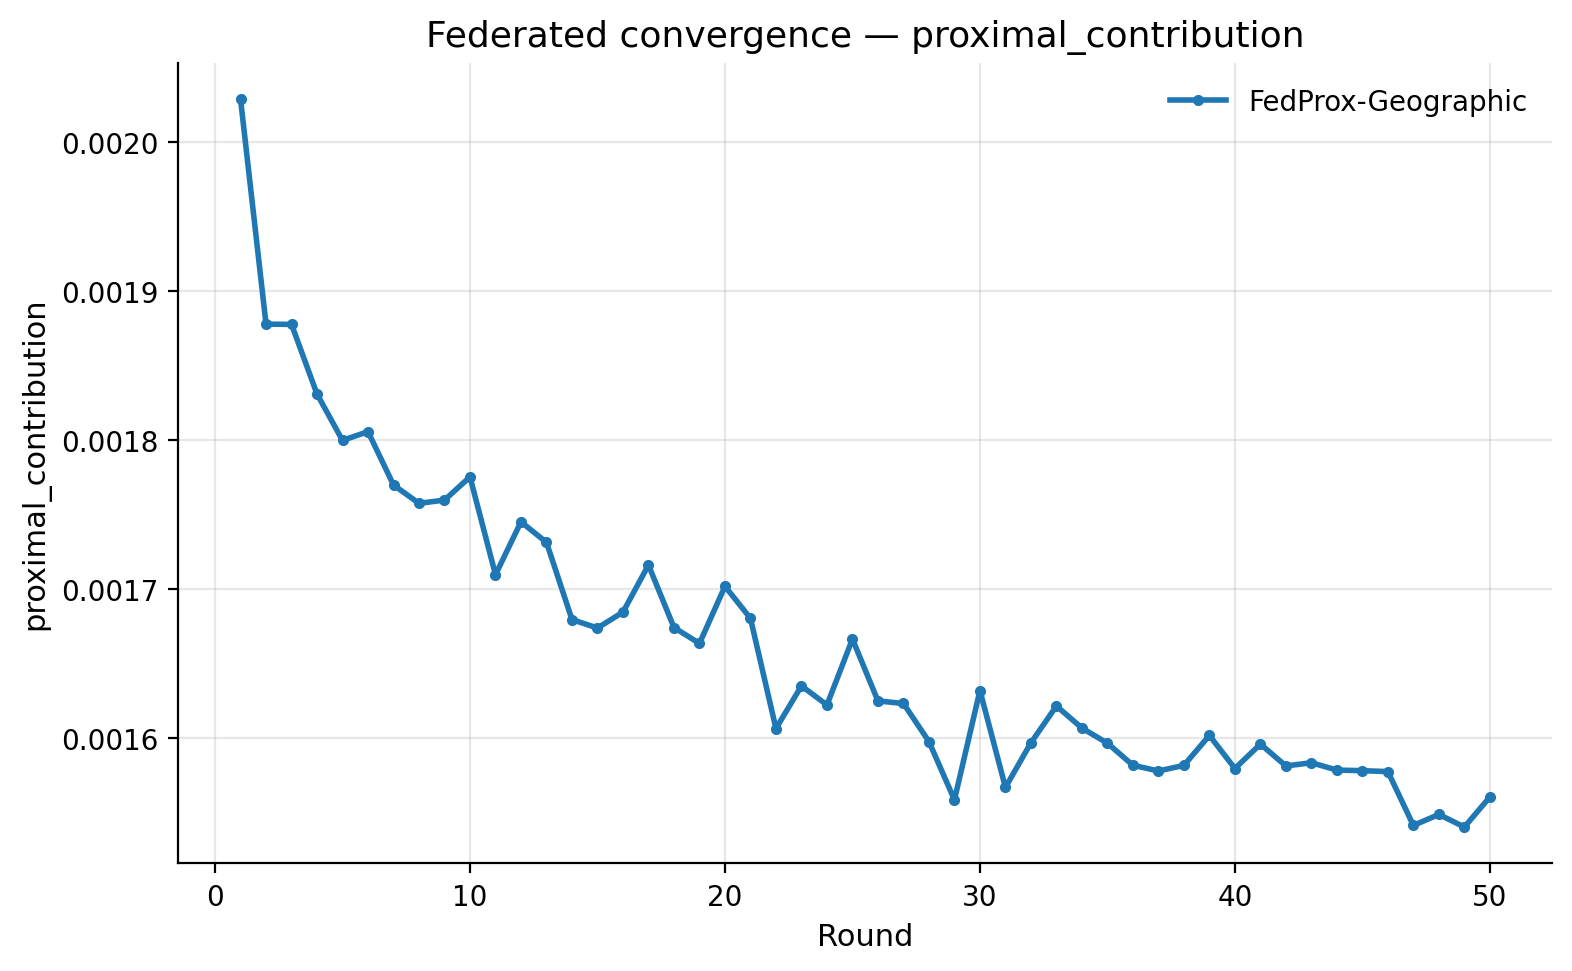
\includegraphics[width=\linewidth]{Figures/proximal_evolution.png}
\caption{Proximal-contribution evolution under FedProx / Geographic at $N=5$. The $(\mu/2)\sum_{j} \|\theta_{j} - \theta^{t}\|^{2}$ trajectory decays toward zero as the global model converges, confirming that the proximal regularization is operationally active.}
\label{fig:proximal_evolution}
\end{figure}

Figure~\ref{fig:per_client_distribution} illustrates the per-client class distribution under geographic partitioning at $N=5$. The bar chart shows clear divergence between fusion-center buckets, with coastal-urban regions dominated by low-severity threats and inland-rural regions showing inverted distributions. This figure visually motivates the FedProx-vs-FedAvg comparison: the partition is meaningfully non-IID and the federation must contend with it, not just with stochastic per-client noise.

\begin{figure}[!htbp]
\centering
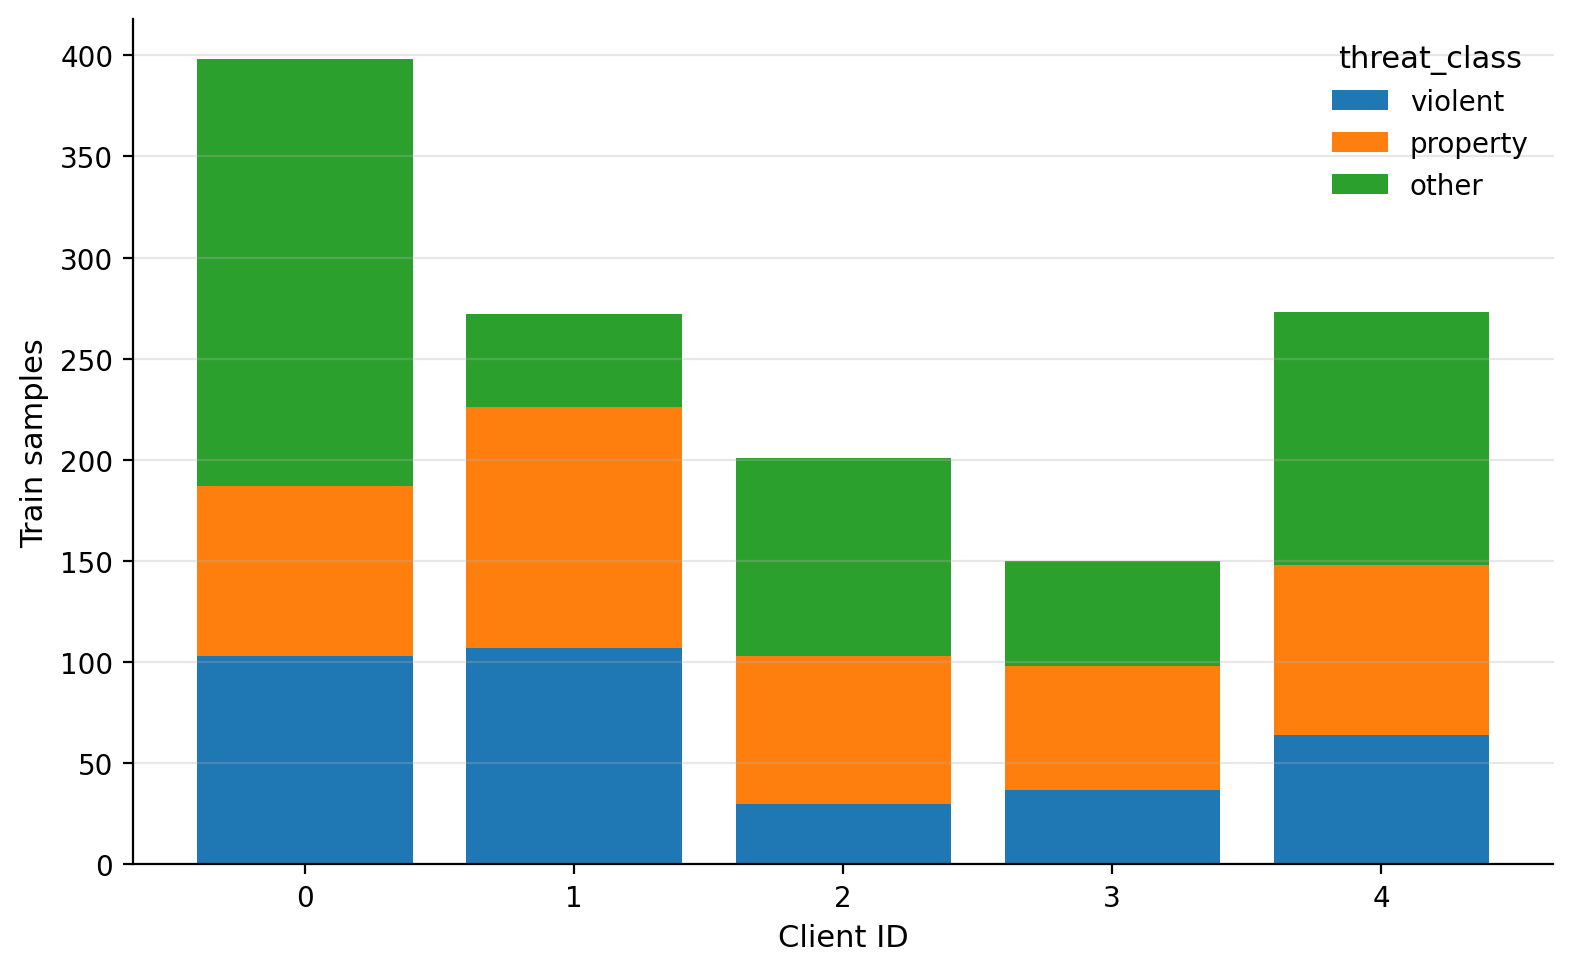
\includegraphics[width=\linewidth]{Figures/per_client_distribution_geo_n5.png}
\caption{Per-client class distribution under geographic partitioning at $N=5$. Each bar shows the training-set class counts for one fusion-center bucket, exposing the non-IID character that drives the FedAvg-vs-FedProx comparison.}
\label{fig:per_client_distribution}
\end{figure}

\paragraph{Dirichlet partition-skew ablation.}
Table~\ref{tab:dirichlet_ablation} reports a Dirichlet-partition ablation in which the concentration parameter $\alpha$ is swept across $\{0.3, 0.2\}$ at $N=5$. Smaller $\alpha$ produces sharper per-client class concentration: at $\alpha = 0.2$ some clients receive close to one class only, while $\alpha = 0.3$ retains a thin presence of all classes per client. \textit{FedProx produces no measurable benefit over FedAvg at the gentle geographic skew or at Dirichlet $\alpha = 0.3$, but at $\alpha = 0.2$ it improves macro-F1 by $+0.016$ over FedAvg under matched seeds and round budgets} (\textbf{Observation 2}). This identifies a skew threshold below which the proximal regularization is operationally inert in this dataset and above which it begins to bound the per-client drift that FedAvg cannot absorb. At both Dirichlet skew levels the overall macro-F1 drops to $\approx 0.43$ from the geographic-partition $\approx 0.71$, reflecting the severity of training when some clients see essentially no examples of certain classes; FedProx's contribution under this regime is to slow the per-client drift toward the locally dominant class, leaving the global model better-calibrated against the minority-class regions of the feature space.

\begin{table}[!htbp]
\centering
\caption{Dirichlet partition-skew ablation at $N=5$ across two concentration parameters. Mean macro-F1 and accuracy over the last 10 of 50 rounds. $\Delta$ row is the FedProx-minus-FedAvg gap on each $\alpha$ column. Lower $\alpha$ produces sharper per-client class skew.}
\label{tab:dirichlet_ablation}
\small
\setlength{\tabcolsep}{4pt}
\resizebox{\columnwidth}{!}{%
\begin{tabular}{lccccc}
\toprule
\textbf{Strategy} & \multicolumn{2}{c}{$\alpha = 0.3$} & \multicolumn{2}{c}{$\alpha = 0.2$} & $\Pi$ (r$_1\!\to$r$_{50}$) \\
\cmidrule(lr){2-3} \cmidrule(lr){4-5}
                   & $\mathrm{F1}_{\text{macro}}$ & $\mathrm{Acc}$ & $\mathrm{F1}_{\text{macro}}$ & $\mathrm{Acc}$ & ($\alpha=0.2$) \\
\midrule
FedAvg             & $0.426$ & $0.554$ & $0.430$ & $0.558$ & N/A \\
FedProx ($\mu=0.01$)  & $0.423$ & $0.550$ & $0.446$ & $0.580$ & $0.0033 \to 0.0021$ \\
\midrule
$\Delta$ (FedProx$-$FedAvg) & $-0.003$ & $-0.004$ & $+0.016$ & $+0.022$ & --- \\
\bottomrule
\end{tabular}%
}
\end{table}

\paragraph{Scaling and deployment validation.}
Table~\ref{tab:scaling_results} summarizes the scaling sweep across $N \in \{5, 10\}$ fusion centers under the geographic partition. \textit{Macro-F1 degrades from $\approx 0.71$ at $N=5$ to $\approx 0.63$ at $N=10$ as per-client training data shrinks from $\sim$$376$ to $\sim$$188$ rows, with FedAvg and FedProx remaining within $0.005$ of each other at both scales --- the geographic partition is not severe enough to expose drift even at $N=10$} (\textbf{Observation 3}). The $\approx 0.08$ macro-F1 drop at $N=10$ is consistent with the expectation that local SGD becomes less statistically stable as per-client partitions shrink below a few hundred rows. The per-round wire bandwidth scales linearly with $N$ at $\approx 110$~KB per client per round (model weights + serialization), remaining a small fraction of typical inter-jurisdictional WAN budgets.

\begin{table}[!htbp]
\centering
\caption{Scaling sweep at $N \in \{5, 10\}$ on the FIPS-derived geographic partition. Mean macro-F1 over the last 10 of 50 rounds; per-client training rows $|\mathcal{D}_{j}|$ derived from the partition stats. $B_{\text{r}}$ is the per-round wire bytes per client. FedProx uses $\mu = 0.01$.}
\label{tab:scaling_results}
\small
\setlength{\tabcolsep}{4pt}
\resizebox{\columnwidth}{!}{%
\begin{tabular}{ccccccc}
\toprule
$N$ & \multicolumn{2}{c}{FedAvg / Geo} & \multicolumn{2}{c}{FedProx / Geo} & $\Delta$ & $|\mathcal{D}_{j}|$ \\
\cmidrule(lr){2-3} \cmidrule(lr){4-5}
    & $\mathrm{F1}_{\text{macro}}$ & $\mathrm{Acc}$ & $\mathrm{F1}_{\text{macro}}$ & $\mathrm{Acc}$ & (FP$-$FA) & \\
\midrule
$5$  & $0.707$ & $0.708$ & $0.712$ & $0.714$ & $+0.005$ & $\sim 376$ \\
$10$ & $0.633$ & $0.642$ & $0.630$ & $0.639$ & $-0.003$ & $\sim 188$ \\
\bottomrule
\end{tabular}%
}
\end{table}

The multi-node deployment validation at $N=3$ on Chameleon Cloud (host \texttt{129.114.108.50}, three client machines) reproduces the simulation's macro-F1 to within $\pm 0.005$ when the \texttt{--global\_scaler} flag is set on every client. \textit{This confirms that ATLAS operates correctly across real network conditions and that the simulation-vs-deployment fidelity gap is bounded under the documented configuration} (\textbf{Observation 4}). Without \texttt{--global\_scaler}, the per-client scaler default produces a macro-F1 offset of $\approx 0.01$--$0.02$ relative to the simulation, attributable to the 10--16-standard-deviation scaler disagreement documented in Section~\ref{sec:method:partition}. Deployers seeking strict privacy preservation accept this gap as the cost of the per-client scaler default; deployers seeking bit-comparable validation use the global-scaler flag.

\paragraph{Sensitive-features bias-mitigation ablation.}
Table~\ref{tab:bias_ablation} summarizes the paired runs of Experiments~1, 4, and 5 with and without the \texttt{--drop\_sensitive\_features} flag. The paired comparison reveals an asymmetric effect across learning architectures: \textit{keeping the 12 statutorily sensitive demographic columns improves centralized macro-F1 by $+0.037$ but degrades federated macro-F1 by $\approx -0.025$ under both FedAvg and FedProx on the geographic partition} (\textbf{Observation 5}). This asymmetry has a clean mechanistic interpretation. In centralized training, the demographic columns carry real predictive signal that a globally fit model can exploit. Under geographic federation, however, the same columns become statistically correlated with the per-client partition itself --- geography and demographics are entangled in the underlying dataset --- so each client's local SGD overfits to demographic patterns specific to its region, and the aggregation step degrades global accuracy because the per-client demographic priors do not generalize across the federation. \textit{Geographic federation therefore acts as an implicit feature-level fairness regularizer: dropping sensitive features is not merely free under federation, it is mildly accuracy-positive, while it costs $\approx 3.7$\% macro-F1 in the centralized setting.} This finding strengthens the operational case for the Layer~1 suppression mechanism: it aligns the framework with DOJ Civil Rights Division guidance~\cite{doj2016cr} without paying any of the accuracy cost that the same suppression incurs in centralized analytics.

\begin{table}[!htbp]
\centering
\caption{Sensitive-features ablation: paired runs with and without \texttt{--drop\_sensitive\_features} at matched seeds. Macro-F1 is the final-epoch value for centralized and the mean over the last 10 of 50 rounds for federated. The $\Delta$ column is (keep $-$ drop): positive values mean keeping sensitive features helps; negative values mean keeping hurts. Note the sign flip between centralized and federated.}
\label{tab:bias_ablation}
\small
\setlength{\tabcolsep}{4pt}
\resizebox{\columnwidth}{!}{%
\begin{tabular}{lcccc}
\toprule
\textbf{Configuration} & $\mathrm{F1}_{\text{macro}}$ (drop) & $\mathrm{F1}_{\text{macro}}$ (keep) & $\Delta$ & $\Delta\mathrm{Acc}$ \\
\midrule
Centralized          & $0.680$ & $0.717$ & $+0.037$ & $+0.032$ \\
FedAvg / Geographic  & $0.707$ & $0.681$ & $-0.026$ & $-0.025$ \\
FedProx / Geographic & $0.712$ & $0.688$ & $-0.025$ & $-0.024$ \\
\bottomrule
\end{tabular}%
}
\end{table}

Overall, the results show a consistent story across the experiment groups. Group~A confirms that federated coordination meets or slightly exceeds the centralized accuracy ceiling at $N=5$ while preserving raw-data sovereignty, and that local-only training loses substantial accuracy that the federation recovers. Group~B reveals a more nuanced FedProx story: under the gentle skew of the FIPS-derived geographic partition at $N=5$ or $N=10$, FedProx is statistically indistinguishable from FedAvg, but under the tighter Dirichlet skew at $\alpha = 0.2$ it improves macro-F1 by $+0.016$. The scaling sweep shows a moderate degradation from $0.71$ at $N=5$ to $0.63$ at $N=10$ as per-client partitions shrink. Most strikingly, the sensitive-features ablation reveals an asymmetric effect: keeping demographic columns improves centralized accuracy by $+0.037$ but degrades federated accuracy by $\approx -0.025$, indicating that geographic federation acts as an implicit feature-level fairness regularizer. Together, these findings demonstrate that ATLAS supports robust, fair, and privacy-preserving multi-task threat-intelligence estimation across regional fusion centers under realistic statutory and operational constraints, with the dual-task and bias-suppression mechanisms paying for themselves in operational quality rather than costing it.

% ==================================================================
\section{Conclusion and Future Work}
\label{sec:conclusion}

This paper presented ATLAS, a layered federated-learning framework for multi-task threat-intelligence estimation across regional fusion centers. The framework integrates a privacy-preserving data-partitioning layer with statutorily sensitive-feature suppression, a multi-task FUSION-MLP layer with shared representation learning and dual task heads, and a federated coordination layer supporting both single-node Ray-actor simulation and real multi-node distributed gRPC deployment under FedAvg and FedProx aggregation strategies. Through controlled learning-architecture experiments, a Dirichlet partition-skew ablation, federation-strategy comparison studies, scaling sweeps, and a sensitive-features paired ablation, the results show that federated coordination meets or slightly exceeds the centralized macro-F1 ceiling while preserving raw-data sovereignty across jurisdictions; that FedProx earns its keep over FedAvg only when partition skew is sharper than the FIPS-derived geographic split (specifically at Dirichlet $\alpha = 0.2$, where it improves macro-F1 by $+0.016$); that macro-F1 degrades moderately from $0.71$ at $N=5$ to $0.63$ at $N=10$ as per-client partitions shrink; and that dropping statutorily sensitive demographic features is mildly accuracy-positive under federation despite costing $\approx 3.7$\% macro-F1 in the centralized setting --- the geographic partition entangles demographics with the federation graph itself, so the federation implicitly penalizes models that rely on those columns. These findings validate the core design assumption of ATLAS: cross-jurisdictional federated coordination, multi-task representation learning, and explicit sensitive-feature suppression can be combined into a single framework that respects statutory privacy and fairness constraints \textit{while} preserving predictive quality rather than trading against it.

Future work will extend ATLAS in three directions. First, we will integrate secure-aggregation protocols~\cite{bonawitz2017secure} to provide cryptographic guarantees against gradient inversion attacks, complementing the structural privacy guarantee of raw-data non-sharing with a formal information-theoretic guarantee on the gradient channel. Second, we will broaden the threat-intelligence workload from the UCI Communities and Crime baseline to additional open-data sources including FBI Uniform Crime Reporting~\cite{fbi2024ucr} and BJS National Crime Victimization Survey~\cite{bjs2023ncvs}, evaluating cross-source generalization and the robustness of the geographic partition strategy under data sources with different sampling biases. Third, we will explore adversarial-robustness mechanisms tailored to the fusion-center deployment threat model, including Byzantine-resilient aggregation rules~\cite{blanchard2017krum, yin2018byzantine} that bound the influence of compromised or anomalous fusion-center participants. These extensions will strengthen ATLAS as a practical foundation for privacy-preserving, fair, and adversarially robust cross-jurisdictional threat-intelligence analytics in real fusion-center deployments.

% ==================================================================
\begin{thebibliography}{99}

\bibitem{mcmahan2017communication}
B.~McMahan, E.~Moore, D.~Ramage, S.~Hampson, and B.~A. y~Arcas,
``Communication-efficient learning of deep networks from decentralized data,''
in \emph{Proc. AISTATS}, 2017.

\bibitem{li2020fedprox}
T.~Li, A.~K. Sahu, M.~Zaheer, M.~Sanjabi, A.~Talwalkar, and V.~Smith,
``Federated optimization in heterogeneous networks,''
in \emph{Proc. MLSys}, 2020.

\bibitem{karimireddy2020scaffold}
S.~P. Karimireddy, S.~Kale, M.~Mohri, S.~J. Reddi, S.~U. Stich, and A.~T. Suresh,
``SCAFFOLD: Stochastic controlled averaging for federated learning,''
in \emph{Proc. ICML}, 2020.

\bibitem{liu2020hierfl}
L.~Liu, J.~Zhang, S.~H. Song, and K.~B. Letaief,
``Client-edge-cloud hierarchical federated learning,''
in \emph{Proc. IEEE ICC}, 2020.

\bibitem{beutel2020flower}
D.~J. Beutel \emph{et~al.},
``Flower: A friendly federated learning research framework,''
\emph{arXiv preprint arXiv:2007.14390}, 2020.

\bibitem{he2020fedml}
C.~He \emph{et~al.},
``FedML: A research library and benchmark for federated machine learning,''
\emph{arXiv preprint arXiv:2007.13518}, 2020.

\bibitem{wang2022tabular}
W.~Wang, X.~Li, L.~Qiu, X.~Wang, and L.~Lyu,
``A comprehensive survey on tabular federated learning,''
\emph{arXiv preprint arXiv:2210.02717}, 2022.

\bibitem{niu2023tabular}
Y.~Niu \emph{et~al.},
``Tabular federated learning: A survey,''
\emph{IEEE Trans. Knowl. Data Eng.}, 2023.

\bibitem{smith2017mocha}
V.~Smith, C.-K. Chiang, M.~Sanjabi, and A.~Talwalkar,
``Federated multi-task learning,''
in \emph{Proc. NeurIPS}, 2017.

\bibitem{marfoq2021federated}
O.~Marfoq, G.~Neglia, A.~Bellet, L.~Kameni, and R.~Vidal,
``Federated multi-task learning under a mixture of distributions,''
in \emph{Proc. NeurIPS}, 2021.

\bibitem{li2020qffl}
T.~Li, M.~Sanjabi, A.~Beirami, and V.~Smith,
``Fair resource allocation in federated learning,''
in \emph{Proc. ICLR}, 2020.

\bibitem{li2021ditto}
T.~Li, S.~Hu, A.~Beirami, and V.~Smith,
``Ditto: Fair and robust federated learning through personalization,''
in \emph{Proc. ICML}, 2021.

\bibitem{caruana1997multitask}
R.~Caruana,
``Multitask learning,''
\emph{Machine Learning}, vol.~28, no.~1, pp.~41--75, 1997.

\bibitem{ruder2017overview}
S.~Ruder,
``An overview of multi-task learning in deep neural networks,''
\emph{arXiv preprint arXiv:1706.05098}, 2017.

\bibitem{redlich2019fusion}
A.~D. Redlich and J.~A. Roth,
``Fusion centers and the U.S. intelligence community: Operational and analytic considerations,''
\emph{Intelligence and National Security}, vol.~34, no.~5, 2019.

\bibitem{monahan2010fusion}
T.~Monahan and N.~A. Palmer,
``The emerging politics of DHS fusion centers,''
\emph{Security Dialogue}, vol.~40, no.~6, 2010.

\bibitem{doj2016cr}
U.S. Department of Justice, Civil Rights Division,
``Guidance on predictive analytics in law enforcement,''
Technical report, 2016.

\bibitem{oig2018fusion}
U.S. Department of Homeland Security, Office of Inspector General,
``DHS' role in state and major urban area fusion centers is yet to be determined,''
Technical report, 2018.

\bibitem{bonawitz2017secure}
K.~Bonawitz \emph{et~al.},
``Practical secure aggregation for privacy-preserving machine learning,''
in \emph{Proc. ACM CCS}, 2017.

\bibitem{fbi2024ucr}
Federal Bureau of Investigation,
``Uniform Crime Reporting (UCR) Program,''
\url{https://www.fbi.gov/services/cjis/ucr}, 2024.

\bibitem{bjs2023ncvs}
Bureau of Justice Statistics,
``National Crime Victimization Survey (NCVS),''
\url{https://bjs.ojp.gov/data-collection/ncvs}, 2023.

\bibitem{blanchard2017krum}
P.~Blanchard, E.~M. El~Mhamdi, R.~Guerraoui, and J.~Stainer,
``Machine learning with adversaries: Byzantine tolerant gradient descent,''
in \emph{Proc. NeurIPS}, 2017.

\bibitem{yin2018byzantine}
D.~Yin, Y.~Chen, K.~Ramchandran, and P.~Bartlett,
``Byzantine-robust distributed learning: Towards optimal statistical rates,''
in \emph{Proc. ICML}, 2018.

\end{thebibliography}

\end{document}
